\documentclass[11pt]{article}

% use packages
\usepackage[utf8]{inputenc}
\usepackage{amsmath}
\usepackage{amsthm}
\usepackage{amsfonts}
\usepackage{amscd}
\usepackage{amssymb}
\usepackage{natbib}
\usepackage{url}
\usepackage[table,xcdraw,usenames]{xcolor}
%\usepackage[usenames]{color}

\usepackage{graphicx}
\usepackage{mathtools}
\usepackage{enumitem}
\usepackage{authblk}
\usepackage{bm}
\usepackage{comment}
\usepackage{pdfpages}


\usepackage{hyperref}
\usepackage{caption}
\usepackage{float}
\usepackage[caption = false]{subfig}
\usepackage{tikz}
\usepackage{multirow}
\usepackage[linesnumbered, ruled,vlined]{algorithm2e}
\usepackage{pdflscape}
\usepackage{etoolbox}

%\AtBeginEnvironment{align}{\setcounter{equation}{0}} % https://tex.stackexchange.com/questions/349247/how-do-i-reset-the-counter-in-align

% margin setup
\usepackage{geometry}
\geometry{margin=0.8in}


% function definition
\newcommand{\R}{\mathbb{R}}
\newcommand{\w}{\textbf{w}}
\newcommand{\x}{\textbf{x}}
\newcommand{\dbf}{\textbf{d}}
\newcommand{\y}{\textbf{y}}
\newcommand{\X}{\textbf{X}}
\newcommand{\Y}{\textbf{Y}}
%\newcommand{\L}{\textbf{L}}
\newcommand{\Hist}{\mathcal{H}}
\newcommand{\Prob}{\mathbb{P}}
\def\mbf#1{\mathbf{#1}} % bold but not italic
\def\ind#1{\mathrm{1}(#1)} % indicator function
\newcommand{\simiid}{\stackrel{iid}{\sim}} %[] IID 
\def\where{\text{ where }} % where
\newcommand{\indep}{\perp \!\!\! \perp } % independent symbols
\def\cov#1#2{\mathrm{Cov}(#1, #2)} % covariance 
\def\mrm#1{\mathrm{#1}} % remove math
\newcommand{\reals}{\mathbb{R}} % Real number symbol
\def\t#1{\tilde{#1}} % tilde
\def\normal#1#2{\mathcal{N}(#1,#2)} % normal
\def\mbi#1{\boldsymbol{#1}} % Bold and italic (math bold italic)
\def\v#1{\mbi{#1}} % Vector notation
\def\mc#1{\mathcal{#1}} % mathical
\DeclareMathOperator*{\argmax}{arg\,max} % arg max
\DeclareMathOperator*{\argmin}{arg\,min} % arg min
\def\E{\mathbb{E}} % Expectation symbol
\def\mc#1{\mathcal{#1}}
\def\var#1{\mathrm{Var}(#1)} % Variance symbol
\def\checkmark{\tikz\fill[scale=0.4](0,.35) -- (.25,0) -- (1,.7) -- (.25,.15) -- cycle;} % checkmark
\newcommand\red[1]{{\color{red}#1}}
\def\bs#1{\boldsymbol{#1}}
\def\P{\mathbb{P}}
\def\var{\mathbf{Var}}
\def\naturals{\mathbb{N}}
\def\cp{\overset{p}{\to}}
\def\clt{\overset{\mathcal{L}^2}{\to}}

\setcounter{tocdepth}{4}
\setcounter{secnumdepth}{4}

\newtheorem{corollary}{Corollary}
\newcommand{\ceil}[1]{\lceil #1 \rceil}
\newcommand{\norm}[1]{\left\lVert#1\right\rVert} % A norm with 1 argument
\DeclareMathOperator{\Var}{Var} % Variance symbol

\newtheorem{cor}{Corollary}
\newtheorem{lem}{Lemma}
\newtheorem{thm}{Theorem}
\newtheorem{defn}{Definition}
\newtheorem{prop}{Proposition}
\theoremstyle{definition}
\newtheorem{remark}{Remark}
\hypersetup{
  linkcolor  = blue,
  citecolor  = blue,
  urlcolor   = blue,
  colorlinks = true,
} % color setup

% proof to proposition 
\newenvironment{proof-of-proposition}[1][{}]{\noindent{\bf
    Proof of Proposition {#1}}
  \hspace*{.5em}}{\qed\bigskip\\}
% general proof of corollary
  \newenvironment{proof-of-corollary}[1][{}]{\noindent{\bf
    Proof of Corollary {#1}}
  \hspace*{.5em}}{\qed\bigskip\\}
% general proof of lemma
  \newenvironment{proof-of-lemma}[1][{}]{\noindent{\bf
    Proof of Lemma {#1}}
  \hspace*{.5em}}{\qed\bigskip\\}

\allowdisplaybreaks

\title{Post-shock Volatility Forecasting Using Aggregated Shock Information}
\author{David Lundquist\thanks{davidl11@ilinois.edu}, Daniel Eck\thanks{dje13@illinois.edu} }
\affil{Department of Statistics, University of Illinois at Urbana-Champaign}
\date{Dec 6th, 2023}

\begin{document}

\maketitle

\begin{abstract} 
We develop a novel procedure for forecasting the volatility of a time series under study immediately following an exogenous shock.  Adapting the synthetic prediction framework of \citet{lin2021minimizing}, we exploit series that have experienced similar shocks.  We aggregate their shock-induced excess volatilities by positing the shocks as affine functions of exogenous covariates.  The volatility shocks are modeled as random effects and estimated as fixed effects.  The aggregation of these estimates is done in service of adjusting the $h$-step-ahead GARCH forecast of the time series under study by an additive term.  The adjusted and unadjusted forecasts are evaluated using three families of benchmarks: the unobservable but easily-estimated realized volatility (RV) of the time series under study, implied volatility, and the empirical volatility over horizons of varying length.  We also compare the performance of the adjusted forecast to the performance of the Realized GARCH forecast, which is known to react faster to rapidly-changing volatility than GARCH incorporating implied volatility.   Finally, we combine Realized GARCH modeling with the synthetic prediction framework, using Realized GARCH in both the estimation of random effects as well as the forecast for the time series under study.  Real-world illustrations are provided, as are simulation results suggesting the conditions under which our approach's hyperparameters can be tuned for best performance.
\end{abstract}

\section{Introduction}

The most important stochastic phenomenon of many time series $(P_{t})_{t\in\mathbb{N}}$, especially financial time series, is the volatility of the return series $(r_{t})_{t\in\mathbb{N}}$.  A financial asset's price series and daily return series may exhibit behavior that makes inapplicable and uninterpretable the traditional methods of time series analysis.  In contrast, the return series is scale-free \citep{tsay2005analysis}, easily-interpreted, and often at least weakly stationary.  Yet even if one could model and forecast price series and return series with high accuracy, that would not necessarily tell us much about the variability of such forecasts nor enlighten us about the evolution of the variability of $(P_{t})_{t\in\mathbb{N}}$ over time. Modern portfolio management and theory requires information about at least the first two moments of a return series, if not higher.  For these reasons and others, volatility modeling has come to dominate financial econometrics over the past four decades.  

% COMMENTING OUT THE FOLLOWING PARAGRAPH BECAUSE IT BELONGS IN DISSERTATION ONLY
\begin{comment}
When $(P_{t})_{t\in\mathbb{N}}$ is positive, as one would expect of a price series, the percentage change over any interval of length $k\in\mathbb{N}$ can be approximated by $\text{log}(\frac{P_{t+k}}{P_{t}})$, owing to the fact that for any nonnegative real number y, $\text{log}(y+1)\leq y$.  Equality holds at exactly y = 0, corresponding to the case where $P_{t+k} = P_{t}$.  It is easily verified that the approximation works well when the ratio $\frac{P_{t+k}}{P_{t}} \in (.85,1.15)$, a return absolute value of $15\%$ or less.  The daily log return series $\text{log}(\frac{P_{t+1}}{P_{t}})$, however, not only provides an approximation to the daily return; the logarithm of a price series has the helpful property of being supported on $\mathbb{R}$.  Partly due to that, it earns a pedigree for its role in geometric Brownian motion, the foundation of much of modern financial mathematics, including the Black-Sholes differential equation \citep{tsay2005analysis}.  Additionally, the log transformation is a tried-and-true variance-reduction technique for heteroskedastic data \citep{faraway2016extending} and non-stationary time series.  In many applications, the log-return of a positive time series will allow us to reject the null of a unit-root process using the methods pioneered in \citet{dickey1979distribution} and \citet{dickey1981likelihood}, thus paving the way for the vast family of autoregressive-moving-average models.
\end{comment}

However, no matter how a time series or its transformations are modeled, forecasting in the prescence of exogenous shock events requires a methodological framework that sensibly incorporates relevant information that has yet to manifest in market price or derivative quantities like volatility.  In this setting, regime-change models are of little use because under the assumption of a known exogenous shock, there is no need to estimate a regime-change time, nor is there data following the exogenous shock event to fit a model.  Asymmetric GARCH models were an early attempt to account for fact that negative returns typically beget larger volatility than positive returns \citep{hansen2012realized}.  As a separate problem, GARCH models have been shown slow to adapt to spikes in volatility \citep{andersen2003modeling}.  \citet{engle2002new} explored the use of implied volatility as an exogenous regressor in a GARCH model, that is, using a so-called GARCH-X model \citep{RePEc:pra:mprapa:100301}. \citet{hansen2012realized} propose Realized GARCH, which aims to solve both the asymmetry problem as well as the slow-reaction problem by introducing a ``measurement equation" as a tool for modeling the contribution to the conditional variance made by the market-implied volatility measure.  The key insight is that that the market-implied volatility measure is not independent of the conditional variance posited by the GARCH model.  Therefore, including the external measure must be done in a way that accounts for this dependence.

The approach herein can be viewed as an attempt to sidestep the functional complexity posited by Realized GARCH by substituting modeling assumptions.  Synthetic Volatility Forecasting proceeds under the assumption that similar unscheduled news events occasion volatility shocks arising from a common shock distribution.

\begin{figure}[h]
\begin{center}
  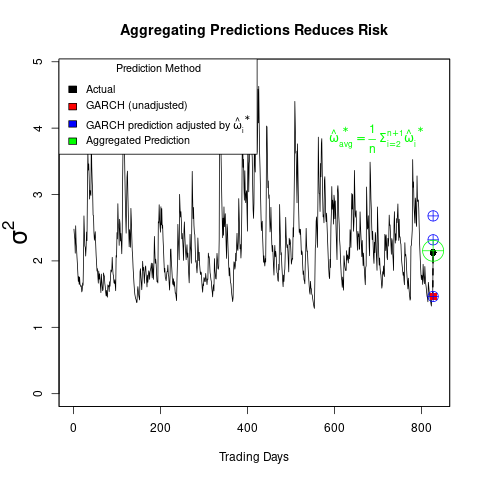
\includegraphics[scale=.5]{simulation_plots/USE_in_paper_simulation_plot_arithmetic_mean.png}
  \caption{A simulated example of shock aggregation using the arithmetic mean of donor fixed effect estimates.}
  \label{fig:arith_mean}
  \end{center}
\end{figure}

As we see in Figure \ref{fig:arith_mean}, the arithmetic mean of estimated shock effects provides perhaps the most straightforward and intuitive way of aggregating information from similar events. Aggregating forecasts using the arithmetic mean is more than merely intuitive; it possesses an empirical pedigree and is known to be optimal under rather restrictive conditions \citep{timmermann2006forecast}.  Synthetic volatility forecasting lacks these restrictions and instead assumes a credible, parsimonious parameterization in which the shock is an affine transformation of several key covariates. \\

\section{Literature Review}

\subsection{Connection to forecast combination methods}
What we are combining, if anything, is subcomponents of forecasts, not forecasts themselves.  However, from a broader perspective, forecast combination is an inapt term for what is being proposed here.  First, the donors are not forecasts. 

\subsection{Why is the proposal here unlike KNN regression?}
In KNN regression, the hyperparameter K must be learned.  In Synthetic Volatility Forecasting, the number of donors is not learned.  A donor pool is curated, and then careful rules of thumb can be applied to determine whether a given donor should be included or excluded. 

\subsection{Should we gather as many donors as possible and pick them quantitatively?}
It would be counter to the method proposed herein to assemble a vast number of donors, lacking careful scrutiny of the qualitative fit, and let the optimization simply pick the donors, via weighting.  What makes a donor good is not merely it's quantitative fit but it's qualitative fit as well.

\subsection{News shock literature review}

We adapt the news shock framework of \citet{kilian2017structural}: \\

$z_{T^{*}+1}^{\text{irregular news shock}} \coloneqq z_{T^{*}+1}^{\text{irregular news}} - \E_{T^{*}}[z_{T^{*}+1}^{\text{irregular news}}]$ \\

In our adapted schema, irregular news shocks are $\mathcal{F}_{T^{*}}$-zero-expectation events governed by a GARCH-X process.  As such, $z_{T^{*}+1}^{\text{irregular news shock}}$ admits of the decomposition $z_{T^{*}+1} = \sigma_{T^{*}+1}\epsilon_{T^{*}+1}$

\subsection{Improvements of this current work over its predecessor}
This present work extends \citet{lin2021minimizing} principally by substituting the GARCH model and for modeling both the mean and volatility of a univariate time series.  We permit both shocks in the mean model and volatility model of GARCH.  As ancillary improvements, the current work permits the shock periods to be of any length, formally $L_{\text{vol}}, L_{\text{level}} \in \mathbb{Z}^{+}$, and the weights applied to the donor pool can come from more exotic subsets of $\mathbb{R}^{n}$.  

At a technical level, the most substantial insight related to \citet{lin2021minimizing} is that the GARCH model provides elegant forecast function for squared observations of the time series under study. To see this, for each $i,t$, define $\eta_{i,t} \coloneqq a^{2}_{i,t} - \sigma^{2}_{i,t}$, and by adding $\eta_{i,t}$ to both sides of the conditional variance specification of $\mc{M}_1$ and $\mc{M}_2$, we obtain the standard ARMA representation of a GARCH(m,s):

\begin{align}
a^{2}_{i,t} = a^{2}_{i,t} - \sigma^{2}_{i,t} + \sigma^{2}_{i,t} = \eta_{i,t} + \sigma^{2}_{i,t} &= \eta_{i,t} + \omega_{i} + \omega^{*}_i D_{i,t}  + \sum^{m_{i}}_{k=1}\alpha_{i,k}a^{2}_{i,t-k} + \sum_{j=1}^{s_{i}}\beta_{i,j}\sigma_{i,t-j}^{2} + \gamma_{i}^{T} \x_{i,t} \\
    &= \eta_{i,t} + \omega_{i} + \omega^{*}_i D_{i,t}  + \sum^{m_{i}}_{k=1}\alpha_{i,k}a^{2}_{i,t-k}  + \sum_{j=1}^{s_{i}}\beta_{i,j}(a^{2}_{i,t-j} - \eta_{i,t-j}) + \gamma_{i}^{T} \x_{i,t} \\
    &= \eta_{i,t} + \omega_{i} + \omega^{*}_i D_{i,t}  + \sum^{\text{max}\{m_{i},s_{i}\}}_{k=1}(\alpha_{i,k} + \beta_{i,k})a^{2}_{i,t-k} - \sum_{j=1}^{s_{i}}\beta_{i,j}\eta_{i,t-j} + \gamma_{i}^{T} \x_{i,t}\label{armarep}
\end{align}

Then for any $i,t$, $\E[a^{2}_{i,t}]$ is nothing more than the expectation of the right-hand side of $(\ref{armarep})$, where $\E[\eta_{i,t}] = 0$ for any $i,t$.  Hence $\E[a^{2}_{i,t}] =  \omega_{i} + \omega^{*}_i D_{i,t}  + \sum^{\text{max}\{m_{i},s_{i}\}}_{k=1}(\alpha_{i,k} + \beta_{i,k})a^{2}_{i,t-k} + \gamma_{i}^{T} \x_{i,t}$

\begin{enumerate}
\item The method under development does not strictly require knowledge of the length of the shocks in the donor pool, but correctly sizing up those shock lengths is helpful to proper estimation of the shocks in the donor pool.  An important question remains: even if the donor pool shock lengths are assumed to be known, how do we advise the operator to forecast the time series under study?  For how long is the forecast reliable?  Should we take a convex combination of the donor pool shock lengths?  Or mean? Or minimum of the donor pool shock lengths?
\item \citet{lin2021minimizing} requires exogenous information to arrive strictly between $T^{*}$ and $T^{*}+1$.  However, we may want to relax this requirement so as to permit the exogenous information to be concurrent with the trading session or end of session on $T^{*}+1$.
\item See Tsay p. 133: if $t$ is the last index that has been observed, then our two-step-ahead forecast is made easier by rewriting the volatility equation as $\sigma^{2}_{i,t+1} = w_{i} + (\alpha_{i} + \beta_{i})\sigma^{2}_{i,t} + \alpha_{1}\sigma^{2}_{i,t}[\epsilon^{2}_{i,t} - 1]= w_{i} + (\alpha_{i} + \beta_{i})\sigma^{2}_{i,t} + \alpha_{1}\sigma^{2}_{i,t}[\epsilon^{2}_{i,t} - 1] $.  Usually, we assume unit variance (though not necessarily a N(0,1)).  However, what is the variance is smaller than 1?  Then in conditional expectation, the term $\alpha_{1}\sigma^{2}_{i,t}[\epsilon^{2}_{i,t} - 1]$ will be negative.  So it seems that for level shock, we want the signal to noise ratio to be large because the mean is high, not because the variance is low.
\end{enumerate}

\section{Setting}
\label{section2}

We follow convention and define the daily log-return as $r_{t} = \text{log}(\frac{P_{t+1}}{P_{t}})$, where $P_{t}$ denotes the price at time $t$.  The class of ARIMA(p,d,q) models developed in the mid-to-late 20th century \citep{box2013box} provides a framework for postulating and quantifying the autoregressive structure of $r_{t}$, all within the framework of frequentist statistics.  These models assume a certain dependence structure between $r_{t}$ and $(r_{k})_{k\leq t}$, yet their errors -- often called innovations in the financial time series context due to how they represent the impact of new information -- are nevertheless assumed to be i.i.d. with mean zero and constant variance.  The ARCH \citep{engle1982autoregressive} and GARCH \citep{bollerslev1986generalized} models provide elegant alternatives to the constant-variance assumption.  In fact, the GARCH framework in its most basic form disregards $r_{t}$ and instead turns its interest to the series $r_{t}^{2}$ (when properly centered, i.e. after assuming a mean-model for returns).  

To that end, let $a_{t} = r_{t} - \mu_{t}$, where $\mu_{t}$ is the mean of the log return series $r_{t}$.  Implicitly, we are committing ourselves to a mean-model for $r_{t}$ in which $\mu_{t}$, the expected daily log-return, may vary with time, while $a_{t}$ is simply the noise.  As \citet{cont2001empirical} explains, such an assumption is justified by the empirical finding that returns lack significant autocorrelation.  We derive a mean-zero process $(a_{t})_{t\in\mathbb{N}}$ with the property that $\E[a^{2}_{t}] = \mrm{Var}[a_{t}]$.  Under the assumption of time-invariant volatility, the series $a_{t}^{2}$ should exhibit no autocorrelation at any lag $\ell\geq1$.  This assumption motivates tests for so-called ARCH effects, that is, tests for the clustering of volatility.  These tests explore the alternative hypothesis that $\sigma_{t}^{2}$ is not only a time-varying parameter but furthermore a function of past squared residuals of the mean model.  In particular, the ARCH(m) model is an autoregressive model in which $\sigma_{t}^{2}$ is fitted using a linear combination of the $m$ past values of $a_{t}^{2}$.  The GARCH(m,s) framework take this one step further but modeling $\sigma_{t}^{2}$ as a linear combination of the $m$ past $a_{t}^{2}$ values and well as the $s$ past values of $\sigma_{t}^{2}$.  In functional form,

\begin{align*}
&\sigma_{t}^{2} = \omega + \sum^{m}_{k=1}\alpha_{k}a^{2}_{t-k} + \sum_{j=1}^{s}\beta_{j}\sigma_{t-j}^{2}\\
&a_{t} = \sigma_{t}\epsilon_{t}
\end{align*}

Assuming further that $\sigma^{2}_{t}$ depends on a vector of exogenous covariates $\x_{t}$ (a so-called ``GARCH-X"), we have

\begin{align*}
&\sigma_{t}^{2} = \omega+ \sum^{m}_{k=1}\alpha_{k}a^{2}_{t-k} + \sum_{j=1}^{s}\beta_{j}\sigma_{t-j}^{2} + \gamma^{T}\x_{t}\\
&a_{t} = \sigma_{t}\epsilon_{t}
\end{align*}


We will suppose that a researcher has multivariate time series data $\y_{i,t}$, $t = 1, \ldots,  T_i$ and $i = 1, \ldots, n+1$. We let $\y_{i,t} = (y_{i,t}$, $\x_{i,t}$, $\textbf{v}_{i,t}$) where $y_{i,t}$ is a scalar response,  $\x_{i,t}$ is a vector of covariates that are revealed to the analyst prior to the observation of $y_{1,t}$, and $\textbf{v}_{i,t}$ is a vector of market-implied volatility metrics for the series $i$ that are available prior to the market open at time t.  Suppose that the analyst is interested in forecasting the volatility of $y_{1,t}$, the first time series in the collection.  We require that each time series $\y_{i,t}$ is subject to a news event immediately following $T^*_i \leq T_i + 1$ and before witnessing $T^*_i+1$. 

In light of the foregoing, we can rewrite the GARCH framework we are interested in as such

\begin{align*}
&\sigma_{i,t}^{2} = \omega_{i} + \sum^{m_{i}}_{k=1}\alpha_{i,k}a^{2}_{i,t-k} + \sum_{j=1}^{s_{i}}\beta_{i,j}\sigma_{i,t-j}^{2} + \gamma_{i}^{T} \begin{pmatrix} \x_{i,t} \\ \textbf{v}_{i,t} \\ \end{pmatrix} \\
&a_{i,t} = \sigma_{i,t}\epsilon_{i,t}
\end{align*}

% https://latex-tutorial.com/matrices-in-latex/
% https://www.math-linux.com/latex-26/faq/latex-faq/article/how-to-write-matrices-in-latex-matrix-pmatrix-bmatrix-vmatrix-vmatrix

We are interested in a point forecast for $\sigma^{2}_{1,T^{*}+h}$, $h=1,2,...,H$, the h-step ahead conditional variance for the time series under study, up to a forecast length of H.  The forecast performance evaluation uses three distinct loss functions, each computed using three families of estimators for the ground truth that we seek.  Let $L^{h}$ with the subscripted pair $\{$prediction method, ground truth estimator$\}$, denote the loss function for an h-step-ahead forecast using a given prediction function and ground truth estimator.  For example, one loss function of interest in this study is the 1-step-ahead MSE using Synthetic Volatility Forecasting and Realized Volatility:

$$ MSE^{1}_{SVF, RV} = (\hat\sigma^{2}_{SVF} - \hat\sigma^{2}_{RV})^{2}$$

In more generality, for an multihorizon volatility forecast with forecast length $H$, the loss function is 

$$ MSE^{H}_{method, ground truth} = \frac{1}{H}\sum_{h=1}^{H}(\hat\sigma^{2}_{h, method} - \hat\sigma^{2}_{h, ground truth})^{2}$$

Also of interest in mean absolute-percentage-error for an h-step-ahead forecast, defined as

\[ 
\text{MAPE}^{H}_{method, ground truth} = \frac{1}{H}\sum_{h=1}^{H}\frac{|\hat\sigma^{2}_{h, method} - \hat\sigma^{2}_{h, ground truth}|}{\hat\sigma^{2}_{h, ground truth}}
\]

Finally, we introduce the QL (quasi-likelihood) Loss \citep{brownlees2011practical}:

\[ 
\text{QL}^{H}_{method, ground truth} = \frac{1}{h}\sum_{h=1}^{H} (\frac{ \hat\sigma^{2}_{h, method} }{\hat\sigma^{2}_{h, ground truth}} - \log{\frac{ \hat\sigma^{2}_{h, method} }{\hat\sigma^{2}_{h, ground truth}}} -1)
\]

What distinguishes QL Loss is that it is multiplicative rather than additive.  This serves as a basis for some of its virtues, both practical and theoretical.  As \citet{brownlees2011practical} explains, ``[a]mid volatility turmoil, large MSE
losses will be a consequence of high volatility without necessarily corresponding to
deterioration of forecasting ability. The QL avoids this ambiguity, making it easier to
compare losses across volatility regimes."


\subsection{Ground Truth Estimators}
\label{Ground Truth Estimators}

The price series of a financial asset is a sequence of observable random variables; in particular, for any $t$, $P_{t}$ is realized at $t$ and henceforth no longer random, under the assumption that $(P_{t})_{t\in\mathbb{N}}$ is adapted to $\mc{F}_{t}$.  Time series econometrics has a vast inventory of approaches for modeling $P_{t}$.  In contrast, the time-varying parameter $\sigma^{2}_{t}$ is a quantity for which even identifying an observable effect in the real world is far more challenging.  Approaches come in two basic forms: model-independent and model-dependent.  The naive approach of constructing a rolling unbiased estimator of the variance of a price series is analogous to using a rolling average to estimate the mean of a price series.  Implicitly, these approaches assume a simple, if unrealistic, covariance structure.  Additionally, they offer very little in the way of forward guidance (predictiveness) regarding the series at hand.  For that reason, in this section, we propose three families of estimators of the ground truth that we aim to forecast.

% https://tex.stackexchange.com/questions/186981/is-there-a-subsubsubsection-command
\subsubsection{Market-Implied Volatility}

Here we introduce implied volatility, a quantity that is derived using the equilibrium price of call and put options on the underlying financial asset.

We note also that Black-Scholes implied volatility is a biased estimator of volatility \citep{mayhew1995implied, christensen1998relation}, with the bias increasing in times of crises when options are out-of-the-money.


\subsubsection{Realized Volatility}

Suppose we examine K units of of time, where each unit is divided into m intervals of length 1/m.  We follow the notation of  \citet{andersen2009realized}. Let $p_{t} = \text{log}(P_{t})$, and let $r(t, 1/m) = p_{t} - p_{t-1/m}$.  We estimate the variance of a log-return series using Realized Volatility, denoted $RV_{K,m}$, using

$$RV_{K,m} = \frac{1}{K}\sum^{Km}_{v=1}r^{2}(v/m,1/m)$$

Assuming that the K units $r(t, 1) = p_{t} - p_{t-1}$ are such that $r(t, 1) \simiid N(\mu, \delta^{2})$, it is easily verified that 

$$\E[RV_{K,m}] = \frac{\mu^{2}}{m} + \delta^{2}$$

which is a biased but consistent estimator of the variance.

\subsubsection{Historical Volatility}

As discussed in section 2, daily returns exhibit insigificant autocorrelation.  Such a finding could be used to motivate using the empirical volatility.  This is just the unbiased estimator of log-return $\sigma^{2}$ over the preceding M days.

\subsection{Volatility Profile of a Time Series}
\label{Volatility Profile of a Time Series}

In this section we make a novel contribution to the synthetic prediction framework by constructing a profile of a time series' volatility.  Suppose we have $D$ donors and for each of those $D$ donors, $q$ distinct measurements and/or covariates of volatility.  Abusing notation for RV ( I need some clever way to index (a) date, (b) donor, (c) how many days were used to get the measurement, we have...

\begin{equation*}
\textbf{V}_{q,D} = 
\begin{pmatrix}
\alpha_{T^{*},1} & \alpha_{T^{*},2}  & \cdots & \alpha_{T^{*},D}  \\
\beta_{T^{*},1} & \beta_{T^{*},2}  & \cdots & \beta_{T^{*},D}  \\
\vdots  & \vdots  & \ddots & \vdots  \\
RV_{T^{*},1} & RV_{T^{*},2}  & \cdots & RV_{T^{*},D}  \\
RV_{T^{*}-1,1}  & RV_{T^{*}-1,2}  & \cdots & RV_{T^{*}-1,D}  \\
\vdots  & \vdots  & \ddots & \vdots  \\
IV_{T^{*},1} & IV_{T^{*},2} & \cdots & IV_{T^{*},D} \\
IV_{T^{*}-1,1}  & IV_{T^{*}-1,2}  & \cdots & IV_{T^{*}-1,D} \\
\vdots  & \vdots  & \ddots & \vdots  \\
AbsoluteReturn_{T^{*},1} & AbsoluteReturn_{T^{*},2} & \cdots & AbsoluteReturn_{T^{*},D} \\
AbsoluteReturn_{T^{*}-1,1}  & AbsoluteReturn_{T^{*}-1,2}  & \cdots & AbsoluteReturn_{T^{*}-1,D} \\
\vdots  & \vdots  & \ddots & \vdots  \\
Volume_{T^{*},1}  & Volume_{T^{*},2}  & \cdots & Volume_{T^{*},D} \\
Volume_{T^{*}-1,1}  & Volume_{T^{*}-1,2}  & \cdots & Volume_{T^{*}-1,D}  \\
\vdots  & \vdots  & \ddots & \vdots  \\
\Delta RV_{T^{*},1} & \Delta RV_{T^{*},2}  & \cdots & \Delta RV_{T^{*},D}  \\
\Delta RV_{T^{*}-1,1}  & \Delta RV_{T^{*}-1,2}  & \cdots & \Delta RV_{T^{*}-1,D}  \\
\vdots  & \vdots  & \ddots & \vdots  \\
\end{pmatrix}
\end{equation*}


\subsection{Aggregation Mechanism}
\label{Aggregation Mechanism}

Here we explain how we use the volatility profile to arrive at a set of nonnegative weights that sum to 1.

In \citet{abadie2010synthetic}, the authors advance previous work in causal inference whereby a treatment effect can be estimated by creating a synthetic time series that that represents either the treatment or control unit.  The synthetic unit is constructed using a convex combination of so-called donor series.  The particular convex combination employed is a function of the distance between the time series under study and the donors. \citet{lin2021minimizing} adapt these methods for the purpose of prediction.  Their 1-step-ahead forecasts take inspiration from distance-based-weighting, pooling shock estimates from similar series according to the series' similarity to the series under study.  The use of fixed-effect estimation for structural shocks has a pedigree (\citet{romer1989does} cited in \citet{kilian2017structural}).  Their approach does not take into account the ARCH effects commonly observed in time series, especially financial times series, leaving unaccounted the variability that accompanies predictions of a heteroskedastic time series.  In this present study, we focus on only volatility forecasting.  We furthermore depart from the synthetic prediction framework by weighting series not by their covariates (which would be most appropriate for estimating the parameters of time series' mean model) but by their volatility profile.


\subsection{Model setup}
\label{modelsetup}
In this section, we will describe the assumed dynamic panel models for which 
post-shock aggregated estimators are provided. The basic structures of these models 
are the same for all time series in the analysis, the differences between them lie in the setup of the shock effect distribution.  We first sharply distinguish between a volatility shock induced by a return series shock and a volatility shock directly affecting the volatility equation of a GARCH model, without mediation of the return series.

\subsubsection{Mean Model and Volatility Model}

Let $I(\cdot)$ be an indicator function, $T_i$ be the time length of the time series $i$ for $i = 1, \ldots, n+1$, and $T_i^*$ denote the largest time index prior to the arrival of the news shock , with $T_i^* < T_i$.  For $t= 1, \ldots, T_i$ and $i = 1, \ldots, n+1$, the model $\mc{M}_1$ is defined as

\begin{align}
\mc{M}_1 \colon &\sigma^{2}_{i,t} = \omega_{i} + \omega^{*}_i D^{vol}_{i,t} + \sum^{m_{i}}_{k=1}\alpha_{i,k}a^{2}_{i,t-k} + \sum_{j=1}^{s_{i}}\beta_{i,j}\sigma_{i,t-j}^{2} + \gamma_{i}^{T} \x_{i,t}\\
&a_{i,t} = \sigma_{i,t}(\epsilon_{i,t}(1-D^{level}_{i,t}) + \epsilon^{*}_{i}D^{level}_{i,t})\\ 
&\omega_i^{*} = \mu_{\omega^{*}} + \varepsilon_{i} \label{model1}
\end{align}

 where $D^{vol}_{i,t} = I(t \in \{T_i^* + 1,...,T_i^* + L_{i, vol}\})$, $D^{level}_{i,t} = I(t \in \{T_i^* + 1,...,T_i^* + L_{i, level}\})$ 
and $\x_{i,t} \in \R^{p}$, with $p \geq 1$.  We assume that the 
$\mbf{x}_{i,t}$ are fixed \footnote{Is this necessary?  Does it serve a purpose?}.\footnote{Need to determine what difference it makes to a GARCH-X model, if any, for the covariates to be random.}\footnote{As for implied volatility as a covariate, the argument for regarding it as a non-random quantity is that we are not primarily concerned with what IV is trying to estimate.  We're concerned with IV itself at a primitive quantity that affects volatility through market sentiment.}  For $i = 1, \ldots, n+1$ and $t=1, \ldots, T_i$, the random effects structure for $\mc{M}_1$ is:

\begin{align*}
  \omega^{*}_i &\simiid \mc{F}_{\omega^{*}} \text{ with }  \; \mrm{E}_{\mc{F}_{\omega^{*}}}(\omega^{*}_i) = \mu_{\omega^{*}}, \mrm{Var}_{\mc{F}_{\omega^{*}}}(\omega^{*}_i)  = \sigma^2_{\omega^{*}}  \\
  \epsilon_{i,t} &\simiid \mc{F}_{\epsilon} \text{ with }  \; \mrm{E}_{\mc{F}_{\epsilon}}(\epsilon) = 0, \mrm{Var}_{\mc{F}_{\epsilon}}(\epsilon)  = \sigma^2_{\epsilon}  \\
  \epsilon^{*}_{i,t} &\simiid \mc{F}_{\epsilon^{*}} \text{ with }  \; \mrm{E}_{\mc{F}_{\epsilon^{*}}}(\epsilon^{*}_{i,t}) = \mu_{\epsilon^{*}}, \mrm{Var}_{\mc{F}_{\epsilon^{*}}}(\epsilon^{*}_i)  = \sigma^2_{\epsilon^{*}}  \\
  % & \text{Alternatively, } (\omega^{*}, \epsilon^{*})_{i} \sim \mathcal{N}(\mu_{\omega^{*},\epsilon^{*}}, \Sigma_{\omega^{*},\epsilon^{*}}) \\
  % THESE ARE NOT RANDOM &(\alpha, \beta)_i \simiid \mc{F}_{(\alpha, \beta)} \text{ where } \sum^{ \text{max} \{m,s \} }_{j}\alpha_j + \beta_j < 1 \\
  % \mathbf{v}_i &\simiid \mc{F}_{\mathbf{v}} \text{ with }  \; \mrm{E}_{\mc{F}_{\mathbf{v}}}(\mathbf{v}_i) = \mu_{\mathbf{v}}, \mrm{Var}_{\mc{F}_{\mathbf{v}}}(\mathbf{v}_i)  = \Sigma^2_{\mathbf{v}} \\
  \varepsilon_{i,t} & \simiid  \mc{F}_{\varepsilon} \text{ with }  \; \mrm{E}_{\mc{F}_{\varepsilon}}(\varepsilon_{i,t}) = 0, \mrm{Var}_{\mc{F}_{\varepsilon}}(\varepsilon_{i,t}) = \sigma^2_{\varepsilon} \\
  %l_{i,vol} &\simiid \text{Unif}\{1,2,...,\text{maximum volatility shock length}\}\\
  %l_{i, level} &\simiid \text{Unif}\{1,2,...,l_{i,vol}\}\\
  \omega^{*}_{i} &\indep \epsilon_{i,t} \indep \epsilon^{*}_{i,t}  \indep \varepsilon_{i,t}.
  \end{align*}

Notice that $\mc{M}_1$ assumes that $\omega^{*}_i$ are i.i.d. with $\E[ \omega^{*}_i]=\mu_{\omega^{*}}$ for $i = 1, \ldots, n+1$. We also consider a model where the shock effects are linear functions of covariates with an additional additive mean-zero error. For $i = 1, \ldots, n+1$, the random effects structure for this model (model $\mc{M}_2$) is:

\begin{align*}
  \mc{M}_2 \colon \begin{array}{l}
     \sigma^{2}_{i,t} = \omega_{i} + \omega^{*}_i D^{vol}_{i,t} + \sum^{m_{i}}_{k=1}\alpha_{i,k}a^{2}_{i,t-k} + \sum_{j=1}^{s_{i}}\beta_{i,j}\sigma_{i,t-j}^{2} + \gamma_{i}^{T} \x_{i,t} \text{ }\\[.2cm]
     a_{i,t} = \sigma_{i,t}(\epsilon_{i,t}(1-D^{level}_{i,t}) + \epsilon^{*}_{i}D^{level}_{i,t})\\[.2cm]
     \omega_i^{*} = \mu_{\omega^{*}}+\delta'\mbf{x}_{i, T_i^*}+ \varepsilon_{i},
  \end{array}
  \end{align*}

  with random effects structure

  \begin{align*}
    \omega^{*}_i &\simiid \mc{F}_{\omega^{*}} \text{ with }  \; \mrm{E}_{\mc{F}_{\omega^{*}}}(\omega^{*}) = \mu_{\omega^{*}}, \mrm{Var}_{\mc{F}_{\omega^{*}_i}}(\omega^{*}_i)  = \sigma^2_{\omega^{*}}  \\
    \epsilon_{i,t} &\simiid \mc{F}_{\epsilon} \text{ with }  \; \mrm{E}_{\mc{F}_{\epsilon}}(\epsilon) = 0, \mrm{Var}_{\mc{F}_{\epsilon}}(\epsilon)  = \sigma^2_{\epsilon}  \\
    \epsilon^{*}_{i,t} &\simiid \mc{F}_{\epsilon^{*}} \text{ with }  \; \mrm{E}_{\mc{F}_{\epsilon^{*}}}(\epsilon^{*}_{i,t}) = \mu_{\epsilon^{*}}, \mrm{Var}_{\mc{F}_{\epsilon^{*}}}(\epsilon^{*}_i)  = \sigma^2_{\epsilon^{*}}  \\
    % & \text{Alternatively, } (\omega^{*}, \epsilon^{*})_{i} \sim \mathcal{N}(\mu_{\omega^{*},\epsilon^{*}}, \Sigma_{\omega^{*},\epsilon^{*}}) \\
    % THESE ARE NOT RANDOM &(\alpha, \beta)_i \simiid \mc{F}_{(\alpha, \beta)} \text{ where } \sum^{ \text{max} \{m,s \} }_{j}\alpha_j + \beta_j < 1 \\
    \delta &\simiid \mc{F}_{\delta} \text{ with }  \; \mrm{E}_{\mc{F}_{\delta}}(\delta) = \mu_{\delta}, \mrm{Var}_{\mc{F}_{\delta}}(\delta_i)  = \Sigma_{\delta} \\
    % \mathbf{v}_i &\simiid \mc{F}_{\mathbf{v}} \text{ with }  \; \mrm{E}_{\mc{F}_{\mathbf{v}}}(\mathbf{v}_i) = \mu_{\mathbf{v}}, \mrm{Var}_{\mc{F}_{\mathbf{v}}}(\mathbf{v}_i)  = \Sigma^2_{\mathbf{v}} \\
    \varepsilon_{i,t} & \simiid  \mc{F}_{\varepsilon} \text{ with }  \; \mrm{E}_{\mc{F}_{\varepsilon}}(\varepsilon_{i,t}) = 0, \mrm{Var}_{\mc{F}_{\varepsilon}}(\varepsilon_{i,t}) = \sigma^2_{\varepsilon}\\
    %l_{i,vol} &\simiid \text{Unif}\{1,2,...,\text{maximum volatility shock length}\}\\
    %l_{i, level} &\simiid \text{Unif}\{1,2,...,l_{i,vol}\}\\
    \omega^{*}_i & \indep  \epsilon_{i,t} \indep  \epsilon^{*}_{i,t} \indep \delta \indep \varepsilon_{i,t}
    \end{align*}

    We further define the parameter sets
    \begin{align}
      \begin{array}{lll}
         \Theta &= &\{(\omega^{*}_i, \epsilon_{i,t}, \epsilon^{*}_{i,t}, \delta,\varepsilon_{i,t})\colon t= 1, \ldots, T_i, i = 2, \ldots, n +1\},\\
         \Theta_{1} &= &\{(\omega^{*}_i, \epsilon_{i,t}, \epsilon^{*}_{i,t}, \varepsilon_{i,t})\colon t= 1, \ldots, T_i, i = 2, \ldots, n +1\},\\
      \end{array}
    \end{align}\label{parameter}
    where $\Theta$ and $\Theta_1$ can be adapted to $\mc{M}_1$ by dropping $\delta$. We assume this for notational simplicity.

\subsection{Properties of Volatility Shock and Shock Estimators}

The model $\mc{M}_1$ is defined by a volatility equation and mean equation, as is any GARCH model.  The choice to model the volatility shock $\omega^{*}_{i}$ as an additive random effect is straightforward.  However, the choice to model the level effect $\epsilon^{*}_{i,t}$ as a temporary rupture in the otherwise i.i.d. sequence of innovations $\epsilon_{i,t}$ stands in need of deeper justification.  One way of arguing for this choice is that, in a discrete time series model, if we assume the arrival of news in the time between $T^{*}$ and $T^{*}+1$, we do not have an easy way to express a conditional distribution of the innovation $\epsilon_{T^{*}+1}$ given the overnight arrival of information.  Using $\epsilon^{*}_{i,t}$ thus breaks this impasse.  This defense also explains why we do not parameterize the level shock at $T^{*}+1$ as a sum of two shocks, $\epsilon_{i,T^{*}+1}$ and $\epsilon^{*}_{i,T^{*}+1}$, which would represent the level shock as generated by two independent sources of stochasticity.  To do so would inelegant and would also lack motivation as a practical level.  While we want to model the shock at $T^{*}+1$ as large in absolute value, we also want to retain the property of a unitary source of noise.

Note that under the popular GARCH(1,1), a dual level-volatility shock has an marginal effect on the conditional variance $\sigma^{2}_{i,t}$ that should be familiar to scholars of GARCH models.  As usual, assume $\alpha+\beta < 1$.  Furthermore, assume that both the volatility shock $\omega^{*}_{i}$ and the level shock $\epsilon^{*}_{i,t}$ are of length one only, and consider a circumstance with no exogenous regressor $\x_{i,t}$. Consider also the case where $r\geq 2$, which is necessary in order to isolate the effects of the level shock $\epsilon^{*}_{i,t}$.  Then

\begin{align}
\sigma^{2}_{i,T^{*}+r+1} & = \omega_{i} + \alpha_{i} a_{T^{*}+r}^{2} + \beta_{i}\sigma^{2}_{i,T^{*}+r} \label{eq0}\\
& = \omega_{i} + \alpha_{i}(\sigma_{i,T^{*}+r}\epsilon_{T^{*}+r})^{2} + \beta_{i}\sigma^{2}_{i,T^{*}+r} \\
& = \omega_{i} + \sigma^{2}_{i,T^{*}+r}(\alpha_{i} (\epsilon_{T^{*}+r})^{2} + \beta_{i})
\end{align}

In (\ref{eq0}), observe that $\omega_{i}^{*}$ and $\epsilon^{*}_{i,t}$ each appear at most once, through the term $\sigma^{2}_{T^{*}+r}$.  This might lead one to suspect  geometric decay of the shocks $\omega_{i}^{*}$ and $\epsilon^{*}_{i}$.  Such a suspicion is easier to substantiate by examining the conditional expectation of the variance, $\mathbb{E}[ \sigma^{2}_{i,T^{*}+r+1} |\mathcal{F}_{T^{*}+r}]$, which also happens to be the principal forecasting tool for a GARCH model \citep{zivot2009practical}.  Indeed, if we assume unit variance for all $\epsilon_{i,t}$ except, of course, $\epsilon^{*}_{i,t}$, then we have 

\begin{align*}
\mathbb{E}[ \sigma^{2}_{i,T^{*}+r+1} |\mathcal{F}_{T^{*}+r}] & = \mathbb{E}[\omega_{i} + \alpha a_{T^{*}+r}^{2} + \beta\sigma^{2}_{i,T^{*}+r} |\mathcal{F}_{T^{*}+r}] \\
& = \omega_{i} + \mathbb{E}[\alpha(\sigma_{i,T^{*}+r}\epsilon_{T^{*}+r})^{2} |\mathcal{F}_{T^{*}+r}] + \beta\sigma^{2}_{i,T^{*}+r} \\
& = \omega_{i} + \alpha\sigma_{i,T^{*}+r}^{2} + \beta\sigma^{2}_{i,T^{*}+r} \tag{Due to the unit variance assumption}\\
& = \omega_{i} + \sigma^{2}_{i,T^{*}+r}(\alpha + \beta) \\
\end{align*}

By repeated substitution, in conditional expectation, the shock is $\mathcal{O}((\alpha+\beta)^{r})$.  We generalize this observation in the following proposition.

\begin{prop}
Let $a_{t}$ be a mean-zero time series obeying a GARCH(1,1) specification with unit-variance errors, all prior to the arrival of a volatility shock of length $L_{\text{vol}} \geq 1$ and level shock of length $L_{\text{level}}\geq 1$ at some time $T^{*}+1$.  Then for any $r$ such that $r \geq \text{max}\{L_{i, vol},L_{i, level}\} + 1$, 

\begin{align}
\mathbb{E}[ \sigma^{2}_{i,T^{*}+r+1} |\mathcal{F}_{T^{*}+r}] & = \omega_{i} + \sigma^{2}_{i,T^{*}+r}(\alpha + \beta) \\
\end{align}
\end{prop}

\begin{proof-of-proposition}
We claim

\begin{align}
\mathbb{E}[ \sigma^{2}_{i,T^{*}+r+1} |\mathcal{F}_{T^{*}+r}] & = \mathbb{E}[\omega_{i} + \alpha a_{T^{*}+r}^{2} + \beta\sigma^{2}_{i,T^{*}+r} |\mathcal{F}_{T^{*}+r}] \label{eq1}\\
& = \omega_{i} + \mathbb{E}[\alpha(\sigma_{i,T^{*}+r}\epsilon_{T^{*}+r})^{2} |\mathcal{F}_{T^{*}+r}] + \beta\sigma^{2}_{i,T^{*}+r} \label{eq2}\\
& = \omega_{i} + \alpha\sigma_{i,T^{*}+r}^{2} + \beta\sigma^{2}_{i,T^{*}+r} \label{eq3}\\
& = \omega_{i} + \sigma^{2}_{i,T^{*}+r}(\alpha + \beta) \label{eq4}
\end{align}

The volatility equation of a GARCH(1,1) dictates that for any $r$, the one-step-ahead volatility is given by the expression inside the expectation in (\ref{eq1}).  By the mean-model assumption of a GARCH(1,1), we have $a_{i,t} = \sigma_{i,t}\epsilon_{i,t}$ and hence by substituting $\sigma_{i,t}\epsilon_{i,t}$ for $a_{i,t}$, we arrive at equation (\ref{eq2}) above.  Using the unit-variance assumption regarding $\epsilon_{T^{*}+r})$, we can compute explicitly the expectation in (\ref{eq3}).  Finally, by rearranging terms, we arrive at equation (\ref{eq4}).
\end{proof-of-proposition}

In other words, for a GARCH(1,1), once two time points removed from the longest shock length, the volatility shock and level shock can be subsumed into one.  However, prior to being two time points removed, there is no such guarantee.  For example, one can take $r = 1$ and level shock of length at least one to see that 

\begin{align}
\mathbb{E}[ \sigma^{2}_{i,T^{*}+r+1} |\mathcal{F}_{T^{*}+r}] & = \mathbb{E}[\omega_{i} + \alpha a_{T^{*}+1}^{2} + \beta\sigma^{2}_{i,T^{*}+1} |\mathcal{F}_{T^{*}+1}] \\
& = \omega_{i} + \mathbb{E}[\alpha(\sigma_{i,T^{*}+r}\epsilon^{*}_{T^{*}+1})^{2} |\mathcal{F}_{T^{*}+1}] + \beta\sigma^{2}_{i,T^{*}+1} \\
& = \omega_{i} + \alpha\sigma^{2}_{i,T^{*}+1}(\mu^{2}_{\epsilon^{*}} + \sigma^{2}_{\epsilon^{*}}) + \beta\sigma^{2}_{i,T^{*}+1} \\
& = \omega_{i} + \sigma^{2}_{i,T^{*}+1}(\alpha(\mu^{2}_{\epsilon^{*}} + \sigma^{2}_{\epsilon^{*}}) + \beta)
\end{align}

 For each of the $p$ entries in $\delta$, the $k$th entry should have the property that
 
 $\mathbb{E}[ x_{i,t,k} \cdot \delta_{k} ] > 0$
 
 In principle, you could have an $\mc{M}_{21}$ shock with a covariate that, in expectation, has a negative marginal contribution to the cumulative shock.

Moreover, after both shocks have been exhausted, their influence disappears quickly.  This short-memory effect has implications for the method being developed herein:

\begin{enumerate}
\item Estimation of effects in donor pool should err on the side of underestimating, not overestimating, the length of the max shock, since overestimation of the shock length brings with it the risk of underestimating $\omega^{*}$.
\item An operator of the method needs some idea of how long the operator expects the shock in the time series under study to be.  Such an idea will guide her trust in the choice of k in the k-step ahead forecast the operator produces.  There are couple of obvious strategies: take all the donors, and over all the donor shock lengths, take the minimium.  Alternatively, one could take the maximum.
\item There may be different risks associated with over/underestimating level shock and vol shock lengths.
\end{enumerate}



In many settings, it is reasonable to model a volatility shock as occuring without a rupture in the mean-zero, i.i.d. sequence $\epsilon_{i,t}$.  In cases like this, outsize movement in the observable random variable $a_{i,t}$ is due solely to the shock $\omega_{i}^{*}$.  Using the ARMA representation of a GARCH(m,s) model, we can see clearly how the random effect $\omega_{i}^{*}$ increases the expectation of the nonnegative random variable $a_{i,t}^{2}$.  The unconditional mean of an ARMA model tells that the random effects simply contribute to the intercept term (see Tsay p. 132):

\begin{align*} 
\mathbb{E}[a^{2}_{i,t}] = \frac{\omega_{i} + \mathbb{E}[\omega_{i}^{*}] }{1 - \sum^{\text{max(m,s)}}_{k=1}(\alpha_{i,k}+\beta_{i,k})}
\end{align*} 

However, since it is not known a priori for which $t$ the effect $\omega_{i}^{*}$ will be nonzero, this fact is of little practical guidance.

\subsection{Unbiasedness of the Synthetic Volatility fixed-effect estimators and Synthetic Volatility prediction functions}

Recall models $\mc{M}_1$ and $\mc{M}_2$:

\begin{align*}
\mc{M}_1 \colon &\sigma^{2}_{i,t} = \omega_{i} + \omega^{*}_i D^{vol}_{i,t} + \sum^{m_{i}}_{k=1}\alpha_{i,k}a^{2}_{i,t-k} + \sum_{j=1}^{s_{i}}\beta_{i,j}\sigma_{i,t-j}^{2} + \gamma_{i}^{T} \x_{i,t}\\
&a_{i,t} = \sigma_{i,t}(\epsilon_{i,t}(1-D^{level}_{i,t}) + \epsilon^{*}_{i}D^{level}_{i,t}) \\
&\omega_i^{*} = \mu_{\omega^{*}} + \varepsilon_{i} \label{model1}
\end{align*}

\begin{align*}
  \mc{M}_2 \colon \begin{array}{l}
     \sigma^{2}_{i,t} = \omega_{i} + \omega^{*}_i D^{vol}_{i,t} + \sum^{m_{i}}_{k=1}\alpha_{i,k}a^{2}_{i,t-k} + \sum_{j=1}^{s_{i}}\beta_{i,j}\sigma_{i,t-j}^{2} + \gamma_{i}^{T} \x_{i,t} \text{ }\\[.2cm]
     a_{i,t} = \sigma_{i,t}(\epsilon_{i,t}(1-D^{level}_{i,t}) + \epsilon^{*}_{i}D^{level}_{i,t})\\[.2cm]
     \omega_i^{*} = \mu_{\omega^{*}}+\delta'\mbf{x}_{i, T_i^*}+ \varepsilon_{i},
  \end{array}
  \end{align*}

We will discuss these two models in the context of a shock in only the volatility, i.e. with $D^{level}_{i,t} \equiv 0$.\\

\citet{abadie2010synthetic} discuss the unbiasedness of SCM estimators in the context of an autoregressive model.  It is well-known that a GARCH(m,s) model has an ARMA representation.  This suggests that, at the very least, when applied to an autoregressive process such an an ARCH model, Synthetic Volatility Forecasting provides an unbiased prediction.  We therefore set out to show three results of increasing difficulty and complexity.

\begin{prop}
Under $\mc{M}_1$ and $\mc{M}_2$, if the volatility series follows an ARCH(1) model, then under the assumptions in \citet{abadie2010synthetic}, $\hat\omega^{*}$ is an unbiased estimator of $\omega_{1}^{*}$.
\end{prop}

\begin{proof-of-proposition}
First, for each $i,t$, define $\eta_{i,t} \coloneqq a^{2}_{i,t} - \sigma^{2}_{i,t}$, and by adding $\eta_{i,t}$ to both sides of the conditional variance specification of $\mc{M}_1$ and $\mc{M}_2$, we obtain the standard ARMA representation of a GARCH(m,s):

\begin{align*}
a^{2}_{i,t} = a^{2}_{i,t} - \sigma^{2}_{i,t} + \sigma^{2}_{i,t} = \eta_{i,t} + \sigma^{2}_{i,t} &= \eta_{i,t} + \omega_{i} + \omega^{*}_i D_{i,t}  + \sum^{m_{i}}_{k=1}\alpha_{i,k}a^{2}_{i,t-k} + \sum_{j=1}^{s_{i}}\beta_{i,j}\sigma_{i,t-j}^{2} + \gamma_{i}^{T} \x_{i,t} \\
    &= \eta_{i,t} + \omega_{i} + \omega^{*}_i D_{i,t}  + \sum^{m_{i}}_{k=1}\alpha_{i,k}a^{2}_{i,t-k}  + \sum_{j=1}^{s_{i}}\beta_{i,j}(a^{2}_{i,t-j} - \eta_{i,t-j}) + \gamma_{i}^{T} \x_{i,t} \\
    &= \eta_{i,t} + \omega_{i} + \omega^{*}_i D_{i,t}  + \sum^{\text{max}\{m_{i},s_{i}\}}_{k=1}(\alpha_{i,k} + \beta_{i,k})a^{2}_{i,t-k} - \sum_{j=1}^{s_{i}}\beta_{i,j}\eta_{i,t-j} + \gamma_{i}^{T} \x_{i,t} \\
\end{align*}

where the $a^{2}_{i,t}$ (the autoregressive terms) are observable and the $\eta_{i,t}$ (the moving average terms) are not.  Next, as shown in \citet{abadie2010synthetic}, under the autoregressive model 

\begin{align*}
  y_{i,t} &= \alpha_{i,t-1}y_{i,t-1} + \beta_{t} \bm{X}_{i,t}  + u_{i,t} \\
 \textbf{X}_{i,t} &= \gamma_{t-1}y_{i,t-1} + \bm{\Pi}_{t-1}\bm{X}_{i,t-1} + \bm{v}_{i,t} 
\end{align*}

and the assumptions that we, the practitioner, choose $\{w_{i}^{*}\}_{2\leq i \leq n + 1}$ such that

\begin{align*}
\begin{array}{lll}
\sum^{n+1}_{i=2}w_{i}^{*}Y_{i,T^{*}} = Y_{1}^{*} & \text{and} & \sum^{n+1}_{i=2}w_{i}^{*}\bm{X}_{i,T^{*}} = X_{1,T^{*}}^{*} \\
\end{array}
\end{align*}\label{Abadie assumptions}

and $u_{i,t}, \bm{v}_{i,t}$ are mean-zero conditional of $\mathcal{F}_{t} = \{Y_{i,t}, \bm{X}_{i,t}\}_{need subscript here}$.

then with even just one pre-treatment period, the synthetic control estimator is unbiased.  Applying this result to Synthetic Volatility Forecasting, assume we choose $\{w_{i}^{*}\}_{2\leq i \leq n + 1}$ such that

\begin{align*}
\begin{array}{lll}
\sum^{n+1}_{i=2}w_{i}^{*}a^{2}_{i,T^{*}} = a^{2}_{1,T^{*}} & \text{and} & \sum^{n+1}_{i=2}w_{i}^{*}\bm{X}_{i,T^{*}} = X_{1,T^{*}}^{*} \\
\end{array}
\end{align*}\label{adapted Abadie assumptions}

Assume further that $\omega_{i} \equiv 0$ in $\mc{M}_1$ and $\mc{M}_2$. Then it follows immediately that under the ARCH(1) model with time-varying parameters, i.e. under the model

\begin{align*}
  a^{2}_{i,t} &= \alpha_{i,t-1}a^{2}_{i,t-1} + \beta_{t} \bm{X}_{i,t}  + u_{i,t} \\
 \textbf{X}_{i,t} &= \gamma_{t-1}a^{2}_{i,t-1} + \bm{\Pi}_{t-1}\bm{X}_{i,t-1} + \bm{v}_{i,t}
\end{align*}

$ \sum^{n+1}_{i=2}w_{i}^{*}a^{2}_{i,T^{*}+1} - a^{2}_{1,T^{*}+1}$ is an unbiased estimator of the news shock.  By inverting the ARMA representation of GARCH(m,s) above, we could recover an unbiased estimator of the news shock $\sum^{n+1}_{i=2}w_{i}^{*}\sigma^{2}_{i,T^{*}+1} - \sigma^{2}_{1,T^{*}+1}$ if we could observe the terms $\sigma^{2}_{i,t}$ or estimate them without bias.  In practice, we do neither.  In particular, we do not observe $a^{2}_{1,T^{*}+1}$ until it is too late, and hence Sythethic Volatility Forecasting approaches the problem from the opposite direction: estimating $\omega^{*}_{1} = \sum^{n+1}_{i=2}w_{i}^{*}\sigma^{2}_{i,T^{*}+1} - \sigma^{2}_{1,T^{*}+1}$ in order to estimate $\sigma^{2}_{1,T^{*}+1}$.  To this end, consider

\begin{align*}
  a^{2}_{i,t} &= \alpha_{i,t-1}a^{2}_{i,t-1} + \beta_{t} \bm{X}_{i,t}  + u_{i,t} \\
 \textbf{X}_{i,t} &= \bm{v}_{i,t} \\
 \beta_{t} & \equiv 0, \forall t \neq T^{*}\\
 \beta_{t} &= \delta, t = T^{*}
\end{align*}

Observe then that $\omega^{*}_{i}$, as defined in $\mc{M}_1$ and $\mc{M}_2$, is subsumed within the model above, where the $\mu_{\omega^{*}}$ term in $\mu_{\omega^{*}}+\delta'\mbf{x}_{i, T_i^*+1}+ \t{\varepsilon}_{i}$ can be accounted for in the first entry of $\bm{X}_{i,T^{*}+1}$ and $\delta$ without loss of generality.  Since each $\omega_{i}^{*}$ is a function of $\bm{X}_{i,T^{*}}$ and a mean-zero noise term, 

\end{proof-of-proposition}

\begin{prop}
Under $\mc{M}_1$ and $\mc{M}_2$,  if the volatility series follows an ARCH(p) model, then under the assumptions in \citet{abadie2010synthetic}, $\hat\omega^{*}$ is an unbiased estimator of $\omega_{1}^{*}$.
\end{prop}

\begin{proof-of-proposition}
Place here
\end{proof-of-proposition}

\begin{prop}
Under $\mc{M}_1$ and $\mc{M}_2$,  if the volatility series follows an GARCH(m,s) model, then under the assumptions in \citet{abadie2010synthetic}, $\hat\omega^{*}$ is an unbiased estimator of $\omega_{1}^{*}$.
\end{prop}

\begin{proof-of-proposition}
Place here
\end{proof-of-proposition}

\subsection{Consistency of the Synthetic Volatility fixed-effect estimators}

Assume
\begin{enumerate}[\itshape]
  \item $\forall i$, $\{a_{i,t}\}_{t=1,...,T_i}$ obeys a GARCH($m,s$) process, where $T_i$ is the length of the $i$th series.
  \item $\forall i, \{X_{i,t}\}_{t=1,...,T_i}$, supported on $\{0,1\}^{T_i}$ is exactly 1 at the shock times $\{T^{*}_{i}+1,...,T^{*}_{i}+k\}$ and exactly zero otherwise.
  \item Let conditions x,y,z in \citet{han2014asymptotic} prevail.
\end{enumerate}

Then $\hat\omega_{i}^{*} \xrightarrow{p} \omega_{i}^{*}$

\begin{proof-of-proposition}
  Place here
  \end{proof-of-proposition}

  \subsection{Consistency of the Synthetic Volatility prediction function}
Here we use the result above to show that $\hat\sigma^{2}_{1,T^{*}+1}\xrightarrow{p}\sigma^{2}_{1,T^{*}+1}$.
\subsection{Why not parameterize the volatility shock as a change in coefficients?}
\begin{enumerate}
\item Swamped by shock: If the goal is near-term forecasting, then we don't really care how those coefficients may be changing.  The assumption is that if any changes occur, their influence cannot account for the large shock. Given that the GARCH parameters for a stationary GARCH process must sum to less than 1, there is an upper bound to the forecastable change.
\item Practically infeasible: If we did that, we would need quite a few time points to reliably estimate the change in the GARCH parameters.  We don't have that.
\end{enumerate}

\begin{table}[]
\begin{tabular}{|p{1.2in}|p{1.9in}|p{1.9in}|}
\hline
  & $\Sigma_{\delta} = I_{p}$ & $\Sigma_{\delta} \neq I_{p}$  \\ \hline
 $\Sigma_{x_{i,T^{*}}} = I_{p}$ & Easiest to model & Captures reasonable possibility of non-zero correlation in random effects \\ \hline
 $\Sigma_{x_{i,T^{*}}} \neq I_{p}$ & Captures empirically-verified phenomenon of non-zero correlation in covariates & Implausibly complicated to model  \\ \hline
\end{tabular}
\end{table}

\subsection{Forecasting}

Here we make reference to Tsay p. 133 and explain, very similarly to Tsay, that the prediction function for a GARCH(m,s) is very similar to an ARMA prediction function.  Modeled after section 2.2 here https://arxiv.org/pdf/2008.11756.pdf

OR we could cite \citet{zivot2009practical}

$\mathbb{E}[ \sigma^{2}_{i,T^{*}+r+1} |\mathcal{F}_{T^{*}+r}]$

\section{Numerical Examples}

Having introduced the model parameters above, we introduce estimation techniques that can be varied

\subsection{Modeling Setup}

\subsection{Peformance Metrics}

\subsection{Most elementary simulation setup}

\subsection{Monte Carlo results}
Recall $\mc{M}_2$:

\begin{align*}
\mc{M}_2 \colon \begin{array}{l}
   \sigma^{2}_{i,t} = \omega_{i} + \omega^{*}_i D^{vol}_{i,t} + \sum^{m_{i}}_{k=1}\alpha_{i,k}a^{2}_{i,t-k} + \sum_{j=1}^{s_{i}}\beta_{i,j}\sigma_{i,t-j}^{2} + \gamma_{i}^{T} \x_{i,t} \text{ }\\[.2cm]
   a_{i,t} = \sigma_{i,t}(\epsilon_{i,t}(1-D^{level}_{i,t}) + \epsilon^{*}_{i}D^{level}_{i,t})\\[.2cm]
   \omega_i^{*} = \mu_{\omega^{*}}+\delta'\mbf{x}_{i, T_i^*}+ \varepsilon_{i},
\end{array}
\end{align*}

\subsubsection{Most elementary simulation setup}

In order to investigate the Synthetic Volatility Forecasting method

\begin{figure}[h!]
\begin{center}
  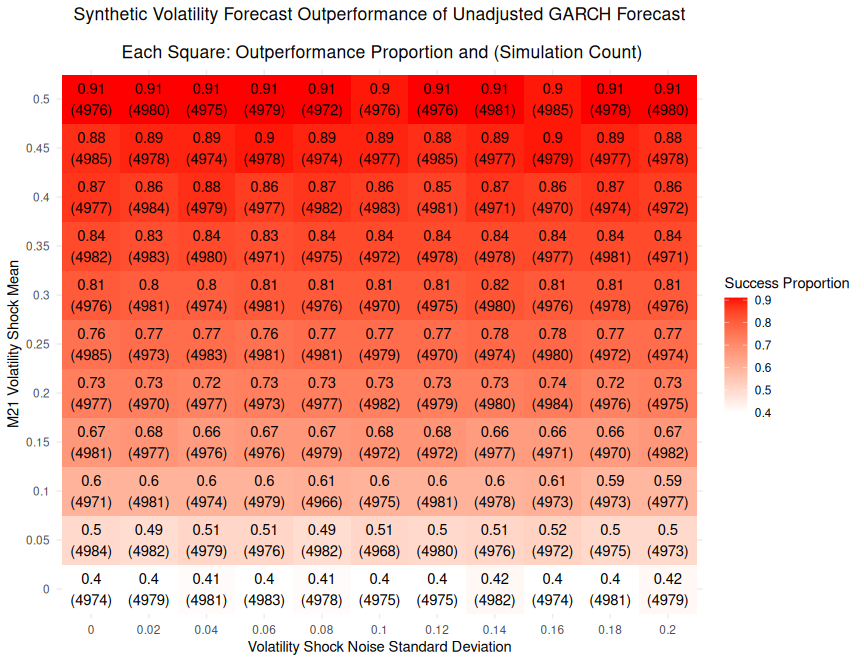
\includegraphics[scale=.45]{simulation_plots/standard_simulation_alpha_.1_beta_.82.png}
  \caption{Fixed parameter values: $\alpha = .1, \beta = .82, \mu_{x} = 1, \sigma_{x} = .1$ (verify)}
  \label{fig:outperformance}
\end{center}
\end{figure}

\begin{figure}[h!]
  \begin{center}
    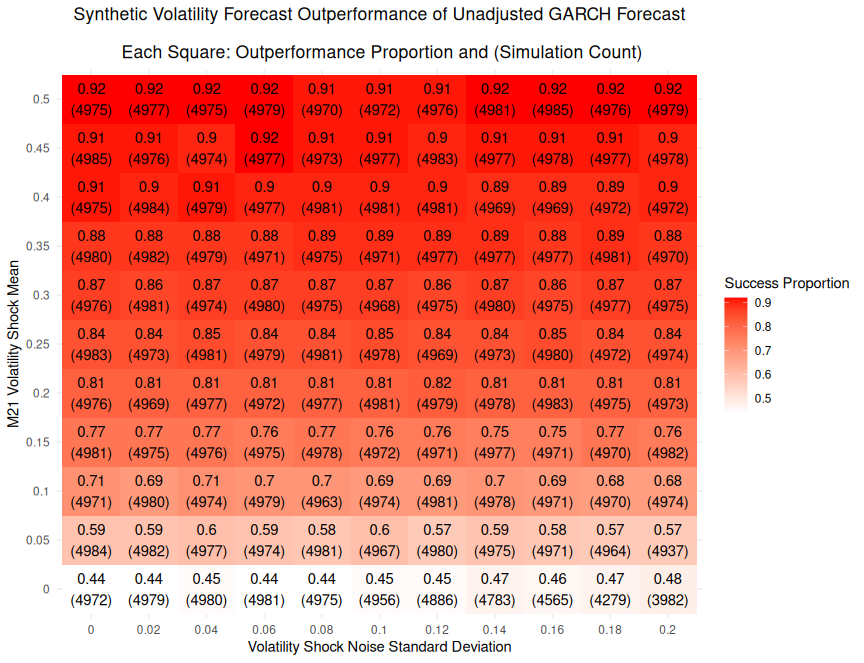
\includegraphics[scale=.45]{simulation_plots/standard_simulation_alpha_.82_beta_.1.png}
    \caption{Fixed parameter values: $\alpha = .82, \beta = .1, \mu_{x} = 1, \sigma_{x} = .1$ (verify)}
    \label{fig:outperformance}
  \end{center}
  \end{figure}
  
As we see in \ref{fig:outperformance}, when only two parameters are varied, the shock signal and the shock noise, we observe several encouraging phenomena:
\begin{itemize}
\item For nearly any row selected in the grid, a pronounced downward trend in the outperformance rate of the SVF exists.
\item For any column selected, an increasing trend exists as the shock signal increases.
\item For almost all small values of the shock signal, the outperformance rate hovers around .5, supporting the hypothesis that in the absence of a signal, any level of noise renders the method anemic.
\end{itemize}

We also introduce simulation parameters that can be varied but are not random effects

\begin{enumerate}
  \item Length of the volatility shock
  \item Length of the level shock
\end{enumerate}


\subsubsection{Dual shock: both a level and volatility shock at $T^{*}+1$}
\textit{Hypothesis:} Method should do less well under level shock.

\begin{figure}[h]
  \begin{center}
    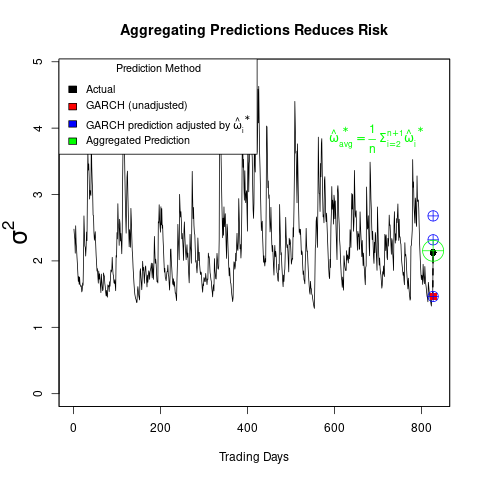
\includegraphics[scale=.5]{simulation_plots/USE_in_paper_simulation_plot_arithmetic_mean.png}
    \caption{Dual shock: both a level and volatility shock at $T^{*}+1$}
    \label{fig:arith_mean}
    \end{center}
  \end{figure}

\subsubsection{Shorter Series}

\subsubsection{Fat tails in innovations}

\subsubsection{Lengthening the measurement period}

\subsubsection{Changing the optimization norm for distance-based weighting}

\subsubsection{Asymmetric GARCH}

\section{Real Data Example}

We show the applicability of Synthetic Volatility Forecasting using a real data example that sits at the crossroads of financial trading and electoral politics.  In the spring of 2016 in the United States, the Republican Party's primary election process narrowed down candidates until Donald J. Trump cleared the threshold of votes to win the nomination formally at the party's convention that summer.  He would go on to face the Democratic Party's nominee, Hillary Rodham Clinton.   

From an ex-ante perspective, several qualities of the 2016 US election cycle as well as the candidates themselves made the election difficult to prognosticate.  The Electoral College permits victory without a majority or even plurality of the popular vote, which can render presidential races more competitive than a raw vote total would, elevating the uncertainty surrounding the country's future leadership.  The election featured no incumbent, ruling out any incumbent-advantage of the empirical, "statistical" kind distinguished by \citet{mayhew2008incumbency}.  The Republican Party candidate espoused unorthodox, populist positions on matters such as healthcare, trade, and foreign policy, some of which could be considered rare in either of the major two parties.  Note here that \citet{goodell2013us} found support for the theory that the polling-implied probabilities of election outcomes encode information about future macroeconomic conditions, which is itself reflected in market volatility.  Additionally, Donald J. Trump, lacking any record in government service -- either electoral or appointed service -- possessed no voting record for voters to judge or his opponents to attack.  

In its final post before the election result, acclaimed forecasting outlet 538, headed by economist Nate Silver, predicted a Clinton victory with a probability of .714, more than 2-to-1 odds \citep{Silver_2016}, suggesting that Trump's victory was at least somewhat surprising.  For these reasons, the aftermath of the 2016 presidential election meets the standard of an interesting and notable event for which a quantitative researcher might seek a volatility point prediction.  On a more technical level, the election outcome was not known until the evening of election day, well after the closing of financial markets at 4pm Eastern Time.  This satisfies the condition that the shock be not yet digested by liquid markets.  We therefore proceed to make the following technical specifications in order to predict the volatility of financial services ETF IYG\footnote{It has been noted that GARCH effects are more attenuated in aggregated returns \citep{zivot2009practical}, which suggests against using the S\&P 500 or similar indices as an example.} (an ETF composed of American financial majors JPMorgan, Bank of American, etcetera) on Wednesday November 9th, 2016.

\begin{enumerate}
    \item \textbf{Model choice} We assume a GARCH(1,1) for the daily log-return series of IYG in each donor.  As argued in \citet{hansen2005forecast}, a GARCH(1,1) is rarely dominated by more heavily-parameterized GARCH specifications.  It thus provides a defensible choice when motivation or time for choosing another model is lacking.  For the time series under study and the donor series alike, we fit a GARCH(1,1) on almost four years of market data prior to the shock.

    \item \textbf{Covariate Choice} We choose covariates that could plausibly satisfy the model assumptions spelled out earlier, that is, risk-related and macroeconomic covariates that could plausibly be weighted and summed in a shock distribution.  We thus choose the log-return Crude Oil (CL.F), the VIX (VIX) and the log-return of the VIX, the log-returns of the 3-month, 5-year, 10-year, and 30-year US Treasuries, as well as the log-return of the spread between AAA and BAA corporate debt, widely considered a proxy for lending risk \citep{goodell2013us, kane1996p}.  We also include the log-return in the trading volume of the ETF IYG itself, which serves as a proxy for panic.  Finally, we include the log-return in British Pound futures (6B=F), partly because we are using Brexit as a donor and partly as a proxy for US dollar strength and investor sentiment.

    \item \textbf{Donor pool construction} Synthetic Control, an a tool of causal inference, often goes about weighting control units by first identifying a natural or set of donors or standard donors such as the untreated units within a set of subnational units like US states or Spanish provinces \citep{abadie2003economic, abadie2010synthetic}.  While such a procedure does not necessarily preclude considered judgments (should Canadian provinces be used as donors for a treated US state?), as a tool of small-n prediction, distanced-based weighting faces a decidedly more difficult task in constructing a donor pool.  
    
    For our purposes, we choose the three most recent US presidential elections prior to the 2016 election as well as the Brexit referendum held in the United Kingdom in May 2016.  The three US presidential elections are the only presidential elections since the advent of the ETF IYG.  We exclude the midterm congressional elections in the US (i.e. those held in even years not divisible by four), which generate far lower voter turnout and feature no national races.   The inclusion of Brexit stands in need of deeper justification because it is non-standard, in the terminology introduced above. Brexit shares with the 2016 presidential race the elements of novel, unorthodox, populist, quasi-isolationist movements in an Anglophone country with a well-developed financial services sector and increasing social division: urban versus rural, colleged-education versus not, cosmopolitan versus versus localist.  Although Euroskepticism and questions of the UK's relationship with continental Europe have a long history in the UK, referenda are not common in British political decision-making, generating uncertainty about the ultimate outcome and its full consequences.  Note that the constituent companies of the IYG, all of which had operations in London, were greatly exposed to the UK's decision to remain or exit the EU.  This explains how an event outside the US financial system can nevertheless be leveraged to study and predict outcomes inside the US.

    \item \textbf{Choice of estimator for volatility} We use the sum of squared 5-minute log-returns of IYG on November 9th, 2016, otherwise known as the Realized Volatility estimator of volatility \citep{andersen2009realized}, as our proxy.  We exclude the first five minutes of the trading day, resulting in 77 sums generated between 9:35am and 4pm.
\end{enumerate} 

\begin{figure}[h!]
\begin{center}
  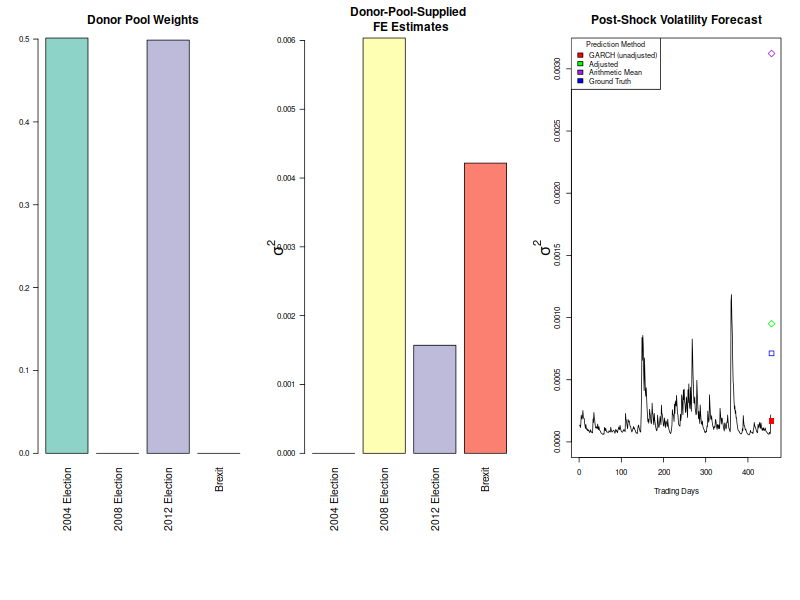
\includegraphics[scale=.6]{real_data_output_plots/savetime_FriOct2707:05:03PM2023_IYG_6B=F-CL=F-^VIX-^IRX-^FVX-^TNX-^TYX_^VIX_2016-11-08-2004-11-02-2008-11-04-2012-11-06-2016-06-23.png}
  \caption{The volatility induced by the 2016 US election}
  \label{fig:SVF_2016}
  \end{center}
\end{figure}

We now discuss the three subplots in Figure \ref{fig:SVF_2016} in order from left to right.  On the left, we see that the distanced-based weighting places nearly equal weight on the 2004 and 2012 elections, with only neglible weight on the 2008 election and Brexit.  Assuming an approximately correct specification of the covariates, this is interpreted to mean that even of the 2016 US election had a general climate of risk and tension less extreme than 2008 and Brexit and more similar to the 2004 and 2012 elections.  In the middle plot, we notice that the fixed effect estimates for 2008, 2012, and Brexit are large, with only 2004 registering a near-zero fixed-effect estimate.  The fixed-effect estimates quantify the amount of surprise the US election results delivered (strictly speaking, not only the presidential race but all November elections in the US with the ability to influence financial markets) under the assumption of a GARCH(1,1).  As estimates gleaned from one data point, they are relatively high in variance.  On the right, we observe in black the fitted values of $\sigma^{2}$ given the GARCH(1,1) for the time series under study.  We also observe four points, all indicated by the legend: three predictions and the ground truth.  We include the prediction derived by adjusting the GARCH(1,1) prediction by the arithmetic mean of the fixed-effect estimates.  As is evident, the Synthetic Volatility Forecasting method comes reasonably close the ground truth.  The prediction is not only directionally correct; it far outperforms the unadjusted prediction.  Remarkably, the arithmetic-mean based prediction here demonstrates the inherent risk in failing to weight each donor appropriately.  The 2008 election and Brexit receive far more weight than is called for because simple averaging ignores the radically different conditons on the even of those two events. \\

Naturally, one would ask how sensitive this prediction is to at least two kinds of model specification: donor pool specification and covariate specification.  There are two responses to these concerns.  First, although the practitioner lacks a priori knowledge of the adequacy of the donors with respect to the time series under study, it is possible to gauge the diversity of the donor information by examining the singular values of the volatility profile.  In the prediction presented here, the no singular value represents more than 50$\%$ of the sum of singular values.  Indeed, the first four singular values descend from 50$\%$ to 25$\%$ to 21$\%$ to 5$\%$ of the the cumulative variation, indicating a low concentration or redundancy of information.  Second, we follow \citet{steegen2016increasing} in a executing a multiverse analysis.  In particular, in the supplement, we carry out leave-one-out analyses on both the donor set and the covariate set.  We here call out that with Brexit removed, the method places nearly all weight on the 2004 election, which has a fixed-effect estimate of almost zero.  Hence, the prediction in \ref{fig:SVF_2016_without_Brexit} outperforms that unadjusted forecast but markedly undershoots the ground truth.

\begin{figure}[h!]
\begin{center}
  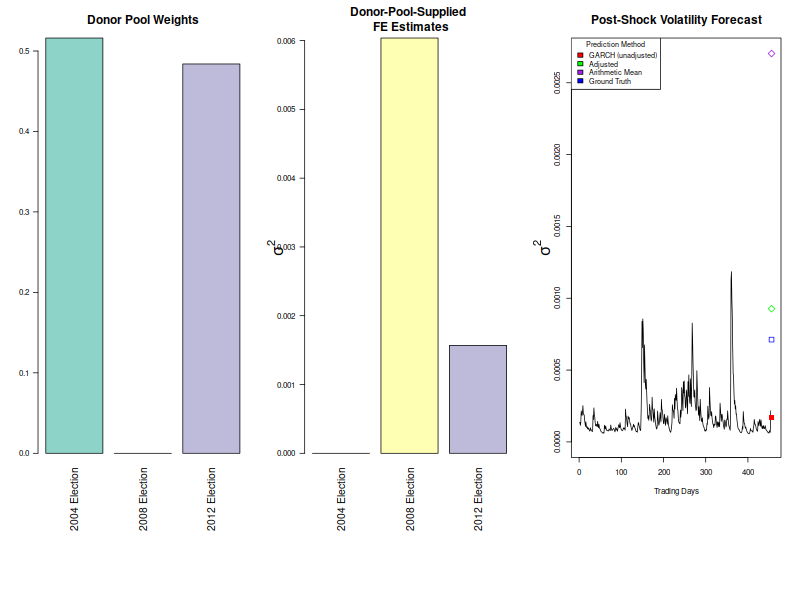
\includegraphics[scale=.6]{real_data_output_plots/savetime_FriOct2707:14:00PM2023_IYG_CL=F-^VIX-^IRX-^FVX-^TNX-^TYX_^VIX_2016-11-08-2004-11-02-2008-11-04-2012-11-06.png}
  \caption{The volatility induced by the 2016 US election, Brexit excluded}
  \label{fig:SVF_2016_without_Brexit}
  \end{center}
\end{figure}

\section{Discussion}

\begin{comment}
\section{Connection to Signal Recovery}

\begin{table}[h!]
\begin{tabular}{|p{1.3in}|p{1.6in}|p{1.9in}|p{1.9in}|}
\hline
 & Vershynin (2018) & Lin and Eck (2021) & SynthVolForecasting \\ \hline
observed quantity& $y_{i}$  & NA & NA \\ \hline
estimated quantity&  NA& $\alpha_{i}$ &  $\omega^{*}_{i}$\\ \hline
signal & $A_{i}x$ & $\mu + \delta'x_{i,T^{*}}$ & $\mu + \delta'x_{i,T^{*}}$  \\ \hline
prior information & $x\in T$, $T$ a convex & across donors, linear shock function equal in distribution  &  across donors, linear shock function equal in distribution \\ \hline
key assumption(s) & $A_{i}$ independent $\forall i$, isotropic too? & $x_{i,T^{*}}$ independent across donors; independent entries of $x_{i,T^{*}}$ & $x_{i,T^{*}}$ independent across donors; independent entries of $x_{i,T^{*}}$ \\ \hline
noise& w & $\t\varepsilon$  & $\t\varepsilon$   \\ \hline
strategy& Observe $y_{i}$; then estimate $x$ with small expected L2 loss & Estimate $\alpha_{i}$ for $i = 2,...,n+1$; then take convex combination to predict $\alpha_{1}$  & Estimate $\omega^{*}_{i}$ for $i = 2,...,n+1$; then take convex combination to predict $\omega^{*}_{1}$ \\ \hline
\end{tabular}
\end{table}

\end{comment}


\section{Supplement}

We analyze the real-world example with Brexit included

\clearpage

\bibliographystyle{plainnat}
\bibliography{synthVolForecast}

  
\end{document}


